\documentclass[aspectratio=1610, 13pt]{beamer}
\usepackage{verbatim}
\usepackage{amsmath}
\usepackage{amsthm}
\usepackage{multicol}
\usepackage{graphics}
\usepackage{color}
\usepackage{stmaryrd}\usefonttheme[onlymath]{serif}

\usepackage{listings}
\usepackage{color}
\renewcommand\lstlistingname{Quelltext} % Change language of section name
\lstset{ % General setup for the package
    language=C,
    basicstyle=\small\sffamily,
    numbers=left,
     numberstyle=\tiny,
    tabsize=4,
    columns=fixed,
    showstringspaces=false,
    showtabs=false,
    commentstyle=\color{red},
    keywordstyle=\color{blue}
}


\title{A Local Shape Analysis based on Separation Logic}
\date{TACAS 2006}
\author{Authors: Dino Distefano, Peter W. O'Heran and Hongseok Yang\\Presentor: Xie Li}
\begin{document}
\maketitle
\begin{frame}{Introduction}
    \begin{center}
        A \textbf{Local} \textbf{Shape Analysis} based on \textbf{Separation Logic}
    \end{center}
    
\begin{itemize}
    \item What is \textbf{Shape Analysis}?
    \item What is \textbf{Separation Logic}?
    \item How the analysis works?
    \item What does \textbf{Local} means?

\end{itemize}
\end{frame}



\begin{frame}{Shape Analysis}
\begin{itemize}
    \item Questions in heap content: NULL-pointers, May-Alias, Must-Alias,  Reachability, Disjointness, \textbf{Shape}.
    
    \item \textbf{Shapes} characterize data structures: singly linked list, linked list with cycle, doubly linked list, a binary tree...
    
    \item According to \footnote{Reinhard Wilheim et al. Shape Analysis. CC 2000.}, shape analysis computes for each point in the program:
    
    A finite, conservative representation of the heap-allocated data structures that could arise when a path to this program point executed.
\end{itemize}
    
\end{frame}

\begin{frame}[fragile]{Shape Analysis: Example}
\begin{multicols}{2}
\begin{example}
    \begin{lstlisting}
    List reverse(List x){
        List y, t;
        y = NULL;
        while(x != NULL){
            t = y;
            y = x;
            x = x->n;
            y->n = NULL;
            y->n = t;
        }
        return y;
    }
    \end{lstlisting}
\end{example}
\emph{Execution state}: cells, connectivity and values of pointer variables.
\begin{center}
    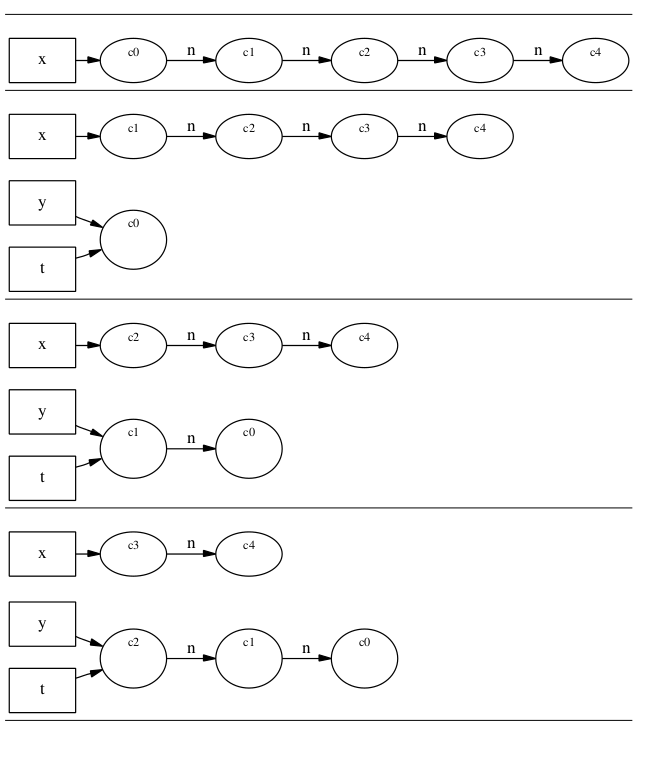
\includegraphics[scale=0.3]{shape_list.png}
\end{center}
\end{multicols}

    
\end{frame}

\iffalse
\begin{frame}{Shape Analysis: Example}
    Shape graph: 
\begin{center}
    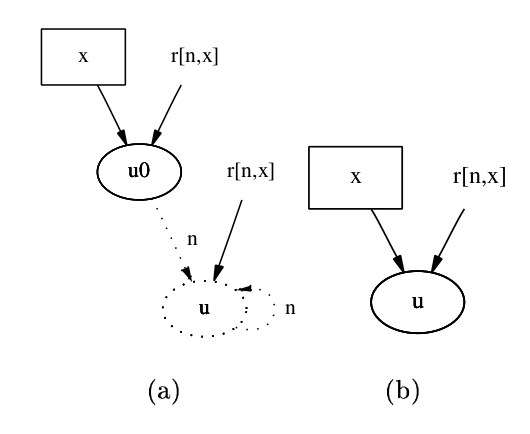
\includegraphics[scale=0.4]{shape_graph.png}
\end{center}
Compute for each program point a set of shape graphs as a description of the superset of execution states at the point.

\end{frame}
\fi
\begin{frame}{Idea of the Paper}
    
    
    
    
    \begin{itemize}
        \item Problem of classic shape analysis: updating of a abstract location may affect properties for other cells. 
        \item Separation logic formula is also capable to express the configuration of memory.
        \item Utilize existing symbolic execution method for separation logic\footnote{Josh Berdine, Cristiano Calcagno and Peter W. O’Hearn. Symbolic execution with separation logic.}.
    \end{itemize}
\end{frame}


\begin{frame}[fragile]\frametitle{Program Considered}
Syntax:

\begin{center}
        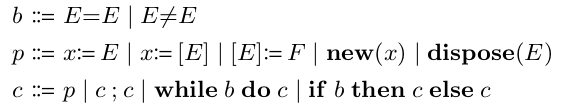
\includegraphics[scale=0.45]{program.png}
    \end{center}

\begin{example}

\begin{align*}
&\mathbf{while}(c\ne 0)  \mathbf{do}\{\\
&t := c;\\
&c := c\rightarrow tl;\\
&\mathbf{dispose}(t);\\
&\}\\
\end{align*}
\end{example}



\end{frame}
\begin{frame}\frametitle{Concrete State Semantic}
	\begin{center}
        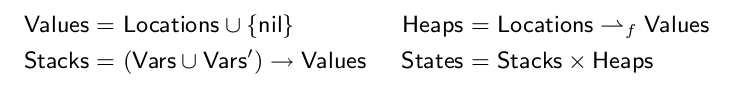
\includegraphics[scale=0.4]{conc_sema.png}
    \end{center}
    Graphically speaking,
    \vspace{10em}
    
    We use $S$ to denote the set $\texttt{States}$.
\end{frame}

\begin{frame}[fragile]\frametitle{Concrete Execution Semantic}
Primitive commands: $x:=E,x:=[E],[E]:=F,\mathbf{new}(x),\mathbf{dispose}(E)$.

Assume the locations and values are all non-negative integers.
\[(s,h), p\Longrightarrow (s',h')\]
\begin{multicols}{2}
\begin{lstlisting}
int main(){

	x = 1;
	
	new(y);
	
	
	[y]:=x;


	dispose(y);
	
}

\end{lstlisting}

\begin{lstlisting}
int main(){

	new(x)
	
	if(x = y){
	
		z := a;
		
	} else {
		z := b;
	}
	dispose(x);
}

\end{lstlisting}\[\mathcal{C}\llbracket c \rrbracket : \mathcal{P}(S) \rightarrow \mathcal{P}(S) \]
\end{multicols}
\end{frame}

\begin{frame}\frametitle{Separation Logic: Symbolic Heap}
\begin{center}
Pure \qquad  Spatial
\end{center}
\huge
\[\Pi \mid \Sigma \]
\small
\vspace{10em}
\begin{center}
        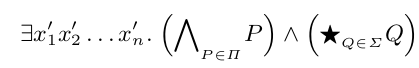
\includegraphics[scale=0.4]{sl_form.png}
    \end{center}
    \[\mathcal{SH}\]
\end{frame}


\begin{frame}\frametitle{Separation Logic: Semantic of Symbolic Heaps}
\begin{example}
    \begin{itemize}
        \item $s,h\models E\mapsto F$: 
        
        $s_0(x) = 1, s_0(y) = 10$ and $h_0(1) = 10$. 
        
        Then $s_0,h_0\models x\mapsto y$.
        \vspace{2em}
        \item $s,h\models \texttt{ls}(E,F)$: intuitively, this means we have a path from $E$ to $F$.
        \begin{itemize}
            \item $s_0(x) = 1, s_0(y) = 10$ and $h_0(1) = 10$. Then $s_0,h_0\models \texttt{ls}(x,y)$
            \item $s_1(x) = 1, s_1(y) = 2, s_1(z) = 3, s_1(w) = 4$ and $h_1(1) = 2, h_1(2)=3, h_1(3) = 4$. Then $s_1, h_1\models \texttt{ls}(x,w)$. Or $s_1, h_1\models x\mapsto y * \texttt{ls}(y,w)$.
        \end{itemize}
        
        \vspace{4em}
        \item $s,h\models \texttt{junk}$ iff $h\ne \emptyset$
    \end{itemize}
    \end{example}
\end{frame}


\begin{frame}[fragile]\frametitle{Symbolic Execution Semantic}
Primitive commands: $x:=E,x:=[E],[E]:=F,\mathbf{new}(x),\mathbf{dispose}(E)$.

Assume the locations and values are all non-negative integers.
\[\Pi\mid \Sigma , p\Longrightarrow \Pi'\mid \Sigma' \]
\begin{multicols}{2}
\begin{lstlisting}
int main(){
	// true|emp
	x = 1;
	
	
	new(y);
	
	
	[y]:=x;


	dispose(y);
	
	
}

\end{lstlisting}
\begin{lstlisting}
int main(){

	new(x)
	
	if(x = y){
	
		z := a;
		
	} else {
		z := b;
	}
	dispose(x);
}

\end{lstlisting}\[\mathcal{I}\llbracket c \rrbracket : \mathcal{P(SH)} \rightarrow \mathcal{P(SH)} \]
\end{multicols}
\end{frame}

\begin{frame}\frametitle{Concretization}

The link between concrete semantic and symbolic semantic:
\large
\[\gamma: \mathcal{P(SH)}\rightarrow\mathcal{P}(\texttt{States})\]
\small

\begin{theorem}
The symbolic semantics is a sound overapproximation of the concrete semantics:
\[\forall X\in \mathcal{P(SH)}. \mathcal{C}\llbracket c\rrbracket(\gamma(X))\subseteq \gamma(\mathcal{I}\llbracket c\rrbracket X)\]
\end{theorem}

\end{frame}

\begin{frame}{General Semantic Setting}
    Working with complete lattice: $D$. 
    
    $D$ is constructed from $\mathcal{P}(S')$, where $S' = S \cup \{\top\}$. $\top$ is a special element corresponds to memory fault.
    
    semantic of a command $\llbracket c\rrbracket: D \rightarrow D$.
    
    \textbf{Semantic for key commands:}
    \begin{center}
        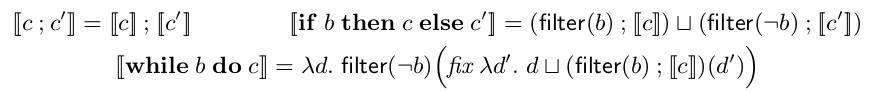
\includegraphics[scale=0.4]{semantic.png}
    \end{center}
    where $\texttt{filter}(b): D \rightarrow D$.
    
    \textbf{Execution semantic:}
    
    $p\Longrightarrow\subseteq S\times(S\cup \{\top\})$
    
    The execution semantic on the powerset of $S'$ is a function $\bar{p}: \mathcal{P}(S') \rightarrow \mathcal{P}(S')$: 
    \[\bar{p} X = \{\sigma'\mid \exists \sigma \in X. (\sigma, p \Longrightarrow \sigma') \vee (\sigma = \sigma' = \top)\}\]
\end{frame}


\iffalse
\begin{frame}{Separation Logic: Concrete and Symbolic Heaps}
    \begin{center}
        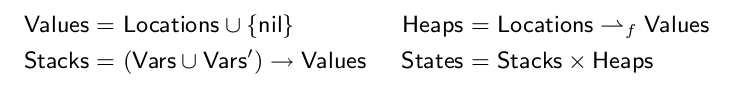
\includegraphics[scale=0.4]{conc_sema.png}
    \end{center}
    \begin{definition}[Symbolic Heap]
    A \emph{symbolic heap} $\Pi\mid \Sigma$ consists of a finite set $\Pi$ of \textbf{equalities} between \textbf{expressions} and a finite set $\Sigma$ of heap predicates, where
    \begin{itemize}
        \item Expressions $E,F$ are variables $x$, primed variables $x'$ or \texttt{nil}.
        \item Heap predicates includes $E\mapsto F$, $\texttt{ls}(E,F)$ and \texttt{junk}.
    \end{itemize}
    \end{definition}
    The meaning of symbolic heap corresponds to a formula:
    \begin{center}
        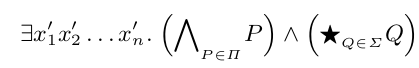
\includegraphics[scale=0.4]{sl_form.png}
    \end{center}
    We use $\mathcal{SH}$ to denote the set of consistent symbolic heaps.
\end{frame}

\begin{frame}{Separation Logic: Concrete and Symbolic Heaps}
Semantic of symbolic heap:
    \begin{example}
    \begin{itemize}
        \item $s,h\models E\mapsto F$: 
        
        $s_0(x) = 1, s_0(y) = 10$ and $h_0(1) = 10$. Then $s_0,h_0\models x\mapsto y$.
        \item $s,h\models \texttt{ls}(E,F)$: intuitively, this means we have a path from $E$ to $F$.
        \begin{itemize}
            \item $s_0(x) = 1, s_0(y) = 10$ and $h_0(1) = 10$. Then $s_0,h_0\models \texttt{ls}(x,y)$
            \item $s_1(x) = 1, s_1(y) = 2, s_1(z) = 3, s_1(w) = 4$ and $h_1(1) = 2, h_1(2)=3, h_1(3) = 4$. Then $s_1, h_1\models \texttt{ls}(x,w)$. Or $s_1, h_1\models x\mapsto y * \texttt{ls}(y,w)$.
        \end{itemize}
        
        
        \item $s,h\models \texttt{junk}$ iff $h\ne \emptyset$
    \end{itemize}
    Or graphically:
    \end{example}
\end{frame}

\begin{frame}{Questions of the Analysis}
The analysis requires us to answer some questions algorithmically:
    \begin{itemize}
        \item $\Pi\vdash E = F$
        
        Check by consider the equivalent classes.
        
        
        
        \item $\Pi\mid \Sigma \vdash \texttt{false}$
        \begin{itemize}
            \item $\Pi\vdash E = \texttt{nil}$ and $\texttt{allocated}(\Sigma, E)$
            \item $\Pi\vdash E = F$ and $\texttt{ls}(E,F)\in \Sigma$
            \item $\Pi\vdash E = F$ and the two distinct predicates whose lhs are $E,F$.
        \end{itemize}
        \item $\Pi\mid \Sigma \vdash E\ne F $ when $\texttt{Vars}'(E, F)=\emptyset$
        
        Add $E = F$ to the pure part and utilize analysis for \texttt{false}.
        
        \item $\Pi\mid \Sigma \vdash \texttt{Allocated}(E)$ when $ \texttt{Vars}'(E)=\emptyset$
    \end{itemize}
    All of the above analysis can be done syntactically.
\end{frame}


\begin{frame}{Questions of the Analysis: Examples}
\begin{example}
    \begin{itemize}
        \item $\Pi\vdash E = F$
        
        Let $\Pi$ be $\{x = x', x' = y', y' = y, z = \texttt{nil}\}$. There are two equivalent classes of the variables: $\{x, x', y, y'\}$ and $\{z, \texttt{nil}\}$. From this information we have $\Pi\vdash x = y$ and $\Pi\vdash z = nil$.
        
        
        
        \item $\Pi\mid \Sigma \vdash \texttt{false}$
        \begin{itemize}
            \item $x = \texttt{nil}\in \Pi$ and $x\mapsto y\in \Sigma$. Inconsistent.
            \item $x = y \in \Pi $ and $\texttt{ls}(x,y)\in \Sigma$. Inconsistent.
            \item $x = y', z\ne y', x = z\in \Pi$. Inconsistent.
        \end{itemize}
        \item $\Pi\mid \Sigma \vdash E\ne F $
        
        Add $E = F$ to the pure part and utilize analysis for \texttt{false}.
        
        \item $\Pi\mid \Sigma \vdash \texttt{Allocated}(E)$
    \end{itemize}
\end{example}
    
\end{frame}
\begin{frame}{Concrete and Symbolic Execution Semantic: Program Considered}
    \begin{center}
        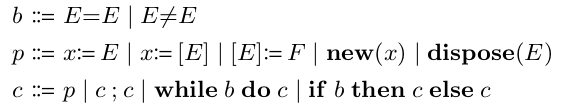
\includegraphics[scale=0.45]{program.png}
    \end{center}
    We use $A(E)$ for any element from the set of primitive commands $\{x:=[E], [E]:=F, \mathbf{dispose}(E)\}$.
    
    With the existing result of \footnote{Josh Berdine et al. Symbolic Execution with Separation Logic}, the author provide the following execution semantics.
\end{frame}


\begin{frame}{Concrete Execution Semantic}
    \begin{center}
        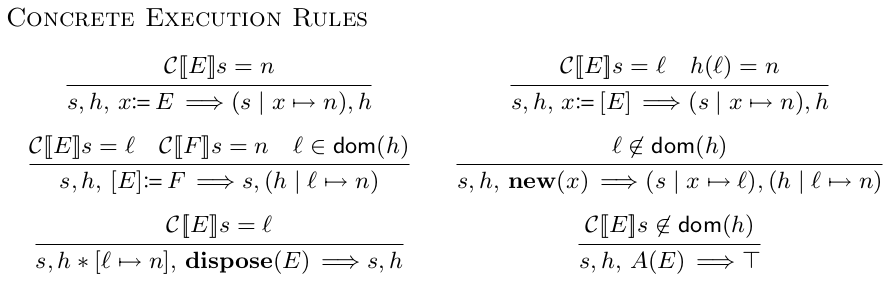
\includegraphics[scale=0.4]{conc_rules.png}
    \end{center}
    The $\sigma$ and $\sigma'$ here in the concrete execution rules are the elements of \texttt{States} defined before.
    
    We extend it to $\mathcal{C}\llbracket c\rrbracket: \mathcal{P}(\mathtt{States})\rightarrow  \mathcal{P}(\mathtt{States})$
    \begin{example}
    An example for the mutation rule:
    
    $s(x) = 10, s(y) = 1$ and $h$ has definition on $10$.
    
    $s, h, [x] := y \Longrightarrow s, (h\mid 10\mapsto 1)$
    
    \end{example}
\end{frame}

\begin{frame}{Symbolic Execution Semantic}
    The symbolic execution semantic $\sigma,p\Longrightarrow \sigma'$, $\sigma$ here is a symbolic heap.
    \begin{center}
        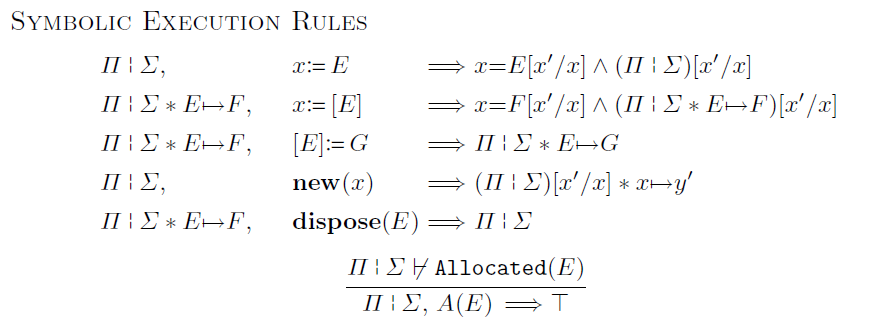
\includegraphics[scale=0.5]{symb_exec.png}
    \end{center}
    These rules also results in an symbolic execution semantic function $\mathcal{I}\llbracket c\rrbracket: \mathcal{P(SH)\rightarrow P(SH)} $.
\end{frame}

\begin{frame}[fragile]{Symbolic Execution Semantic: Example}
\begin{center}
    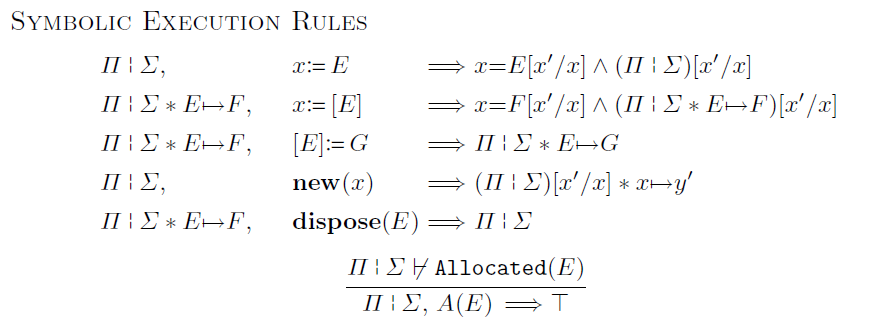
\includegraphics[scale=0.35]{symb_exec.png}
\end{center}
\begin{example}
\begin{center}
    
\begin{multicols}{2}
\begin{lstlisting}
int main(){
    // true|emp
    x = 1;
    // x=x'|emp
    new(y);
    // x=x'|emp * y|->y'
    [y]=x;
    // x=x'|emp * y|->x
    dispose(y);
    // x=x'|emp
    dispose(y);
    // T
}
\end{lstlisting}
\end{multicols}
\end{center}
\end{example}


\end{frame}

\begin{frame}{Rearrangement Rules for \texttt{ls} Predicate}
    \begin{center}
        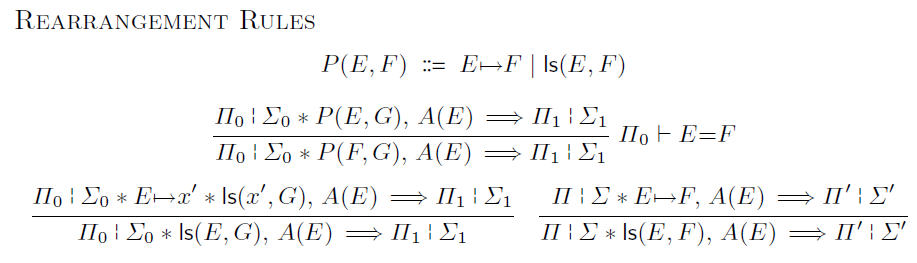
\includegraphics[scale=0.5]{rar.png}
    \end{center}
    
\end{frame}

\begin{frame}{Meaning Function and Safe Semantic}
    To state that the symbolic semantic is sound, we define a \emph{meaning function}:
    \[\gamma: \mathcal{P(SH)}\rightarrow \mathcal{P}(\mathtt{States})\]
    to maps the set of symbolic heap to the set of states that whose elements at least make one of the symbolic heap satisfied.
    
    Then by checking the rules we have
    \begin{theorem}
    The symbolic semantics is a sound overapproximation of the concrete semantics:
    \[\forall X\in \mathcal{P(SH)}. \mathcal{C}\llbracket c\rrbracket(\gamma(X)) \subseteq \gamma(\mathcal{I}\llbracket c\rrbracket X)\]
    
    \end{theorem}
\end{frame}

\fi
\begin{frame}{Problem Encountered}
    \Large
    \begin{center}
    $\mathcal{SH}$ is an infinite set.
    
    \end{center}
    \small
    
    Define an abstract domain for the fix-point convergence and abstraction rules for the conversion.
    \begin{itemize}
        \item Expression replacement for primed variables.
        \item Garbage collection rules.
        \item List abstraction rules.
    \end{itemize}
    The conversion is given by $\leadsto$. The abstract domain after the abstraction is $\mathcal{CSH}$ and corresponding abstract semantic function $\mathcal{A}\llbracket c\rrbracket: \mathcal{P(CSH) \rightarrow P(CSH)}$.
\end{frame}

\begin{frame}{The Analysis}
    \begin{theorem}
    $\mathcal{CSH}$ is finite.
    \end{theorem}
    \begin{theorem}
    The abstract semantic is a sound overapproximation of the concrete semantic.\[\forall X\in \mathcal{P(SH)}. \mathcal{C}\llbracket c\rrbracket(\gamma(X)) \subseteq \gamma(\mathcal{A}\llbracket c\rrbracket X)\]
    \end{theorem}
    
\end{frame}

\begin{frame}\frametitle{The Analysis}
\begin{example}
    A program to dispose a list.
    
    \texttt{Program}: \textbf{while} $(c\ne0)$ \textbf{do} ($t:=c;c:=c\rightarrow tl;\mathbf{dispose(t)}$)
    
    \texttt{Pre:} $\{\}\mid\{\texttt{ls}(c,0)\}$
    
    \texttt{Post:} $\{c=0\}\mid \{\}$
    
    \texttt{Inv:} $\{c=0\}\mid \{\} \vee \{\}\mid \{\texttt{ls}(c,0)\}$
    \end{example}
\end{frame}
\iffalse
\begin{frame}{Locality}
	
    \begin{example}
    Program: $x:=c;c:=c\rightarrow tl$
    
    \texttt{Pre:} $\{\}\mid \{\texttt{ls}(c,d)*d\mapsto d'\}$

    \texttt{Post:} $\{c=d\}\mid \{x\mapsto d *d\mapsto d'\} \vee \{\}\mid \{x\mapsto c* \texttt{ls}(c,d) *d\mapsto d'\}$  
    
    A smaller input provide information we need:
    
    \texttt{Pre:} $\{\}\mid \{\texttt{ls}(c,d)\}$

    \texttt{Post:} $\{c=d\}\mid \{x\mapsto d \} \vee \{\}\mid \{x\mapsto c* \texttt{ls}(c,d) \}$  
    \end{example}
    
    
    The notion of $*$ on symbolic heaps:
    \[(\Pi_1\mid \Sigma_1) *(\Pi_2\mid \Sigma_2) = ((\Pi_1\cup \Pi_2\mid \Sigma_1*\Sigma_2))\]
    
    \begin{theorem}[Frame Rule]
    For all $X,Y\in \mathcal{P(CSH)}$, if $\texttt{Vars}(Y) \cap Mod = \emptyset$ then $\gamma(\mathcal{A}\llbracket c\rrbracket(X*Y)) \subseteq \gamma(\mathcal{A}\llbracket c\rrbracket X)*Y$
    \end{theorem}
\end{frame}
\fi
\begin{frame}{Locality}
	
    \begin{theorem}[Frame Rule]
    For all $X,Y\in \mathcal{P(CSH)}$, if $\texttt{Vars}(Y) \cap Mod(X) = \emptyset$ then $\gamma(\mathcal{A}\llbracket c\rrbracket(X*Y)) \subseteq \gamma(\mathcal{A}\llbracket c\rrbracket X)*Y$
    \end{theorem}
\end{frame}

\begin{frame}\frametitle{Conclusion}

\begin{itemize}
\item Concrete semantic.

\item Symbolic semantic. (Symbolic heap)

\item Abstract semantic. (Canonical symbolic heap)

\item Locality.

\end{itemize}

What can be done with the sound over-approximation?

\end{frame}
\end{document}